%
% Modified by Megan Patnott
% Last Change: Jan 18, 2013
%
%%%%%%%%%%%%%%%%%%%%%%%%%%%%%%%%%%%%%%%%%%%%%%%%%%%%%%%%%%%%%%%%%%%%%%%%
%
% Modified by Sameer Vijay
% Last Change: Tue Jul 26 2005 13:00 CEST
%
%%%%%%%%%%%%%%%%%%%%%%%%%%%%%%%%%%%%%%%%%%%%%%%%%%%%%%%%%%%%%%%%%%%%%%%%
%
% Sample Notre Dame Thesis/Dissertation
% Using Donald Peterson's ndthesis classfile
%
% Written by Jeff Squyres and Don Peterson
%
% Provided by the Information Technology Committee of
%   the Graduate Student Union
%   http://www.gsu.nd.edu/
%
% Nothing in this document is serious except the format.  :-)
%
% If you have any suggestions, comments, questions, please send e-mail
% to: ndthesis@gsu.nd.edu
%
%%%%%%%%%%%%%%%%%%%%%%%%%%%%%%%%%%%%%%%%%%%%%%%%%%%%%%%%%%%%%%%%%%%%%%%%


%
% Chapter 2
%

\chapter{Experimental Setup}
\label{chap:setup}

\section{Overview}

To measure conversion electrons for nuclear structure, three separate experiments were performed at the Nuclear Science Laboratory (NSL) at the University of the Notre Dame using the Internal Conversion Electron Ball (ICEBall) Spectrometer paired with several configurations of High Purity Germanium (HPGe) detectors. A Sm$(\alpha,2n)$Gd reaction was used with different enriched targets to create the desired Gd isotope.

\section{Nuclear Science Laboratory at Notre Dame}

The Nuclear Science Laboratory at the University of Notre Dame has been in operation since the 1930s. Currently, the NSL operates locally with three accelerators: the 10 MV FN Tandem, the 5 MV Sta. Ana accelerator, and the 3 MV 9S Tandem. There is also a fourth accelerator, a 1 MV machine called CASPAR, located in the Homestake Mines in South Dakota. The experiments in this dissertation were performed on the 10 MV FN Tandem. Figure \ref{fig:NSL} is the current layout of the NSL. The accelerator in the top right of the figure is the FN Tandem.

The FN Tandem has two ion sources: the Helium Ion Source (HIS) and the Multi-Cathode Source of Negative Ions Using Cesium Sputtering (MC-SNICS). Most elements can take the electrons from cesium to create negative ions. Helium cannot and needs a special source, as discussed below. For the experiments described, the HIS was used.

Due to the electron binding energy of helium, the HIS uses a duoplasmatron. Within the duoplasmatron, a thin tungsten wire is heated while surrounded by the source gas (helium). The tungsten wire emits electrons, and positively ionizes the helium. This helium is extracted from the duoplasmatron and focused by an einzel lens, where it then goes through the lithium charge exchange. This section of the HIS works much like the Tandem, although the charge exchange works in reverse. The positively charged ions are accelerated through a lithium vapor, and some gain electrons, becoming neutral or negatively charged. Those ions that become negatively charged are accelerated out the other end of the HIS, before being sent to the FN Tandem. Figure \ref{fig:HIS} is a schematic of this system.

\begin{figure}[t]
    \centering
    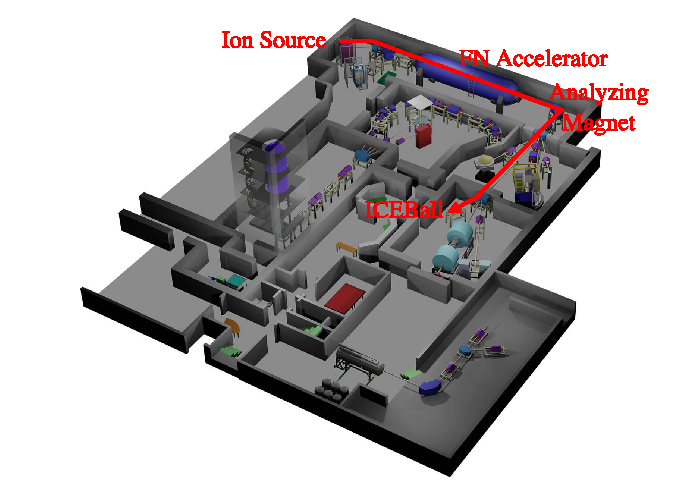
\includegraphics[scale=1.25]{Setup_Figs/NSL_2018_Layout.eps}
    \caption{Current layout of the Nuclear Science Laboratory at Notre Dame. The red line indicates the path taken by the beam, from ion source, through the accelerator and analyzing magnet, before being sent to ICEBall.}
    \label{fig:NSL}
\end{figure}

The 10 MV FN Tandem has been in operation since 1968. It operates using a Van de Graaff system. Charging chains carrying a static charge deposit the charge on a terminal in the center of the machine. The charging chains are a pelletron system, upgraded from the original insulated belt system in 2000. The pelletron chain consists of metal pellets connected using nylon, allowing for each pellet to be electrically isolated as it carries electrical charge to the terminal \citep{nec:_pelletron}. The beamline is kept at vacuum, but the area outside of the beamline, but within the accelerator tank, is filled with a mixture of CO$_2$ and dry nitrogen gas, at approximately 200 PSI. To create a more uniform acceleration field, the terminal is brought to ground along the beamline using resistor-lined tubes. The resistors used create a uniform electrical field down the tube, allowing for uniform acceleration.

It is known as a tandem because the system is a two-stage acceleration. Negatively charged ions enter the system, accelerating toward a positively charged terminal shell. Inside of the shell, the ions go through carbon stripping foils 3 $\mu g/cm^2$ thick, becoming positively charged as electrons are pulled off. The ions then accelerate away from the terminal for the second stage. The total energy gained by the ions is the terminal voltage times the quantity of one plus the final charge state.

\begin{figure}
    \centering
    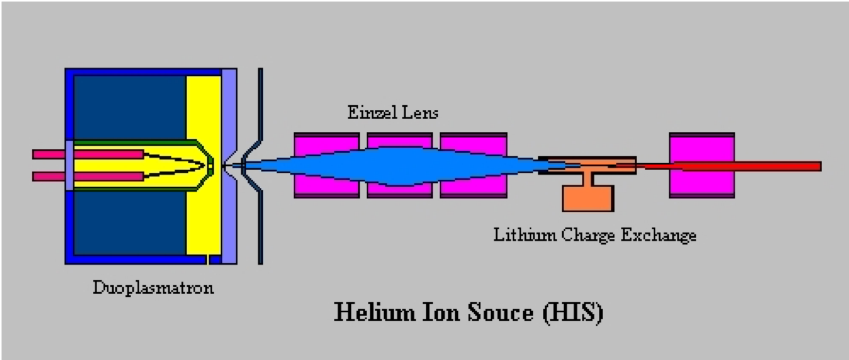
\includegraphics[scale=0.75]{Setup_Figs/HIS.png}
    \caption{A schematic of how the Helium Ion Source works.}
    \label{fig:HIS}
\end{figure}

\section{Target Fabrication}

For conversion electron experiments, thinner targets are ideal. Electrons must escape the target for detection, and a thicker target causes energy loss and straggling effects, blurring out the conversion electron spectrum.

Enriched, self-supporting samarium targets were used for this experiment. Table \ref{tab:target} has the enrichment and thickness of the targets used. The material started as Sm$_2$O$_3$. Using the reaction

\begin{equation}
    Sm_2O_3 + Hf \xrightarrow{} HfO_2 + Sm
    \label{eq:sm_hf}
\end{equation}

at a temperature of 1520-1820 K the samarium was extracted as a metal \citep{clifford02:_target}. Once cooled, it was rolled as thin as possible. Samarium easily oxidizes, stagnating the rolling process, as too much work on the material at once could cause instantaneous oxidization, resulting in the loss of the target. Rolling had to be done incrementally, giving the material time to rest.

\begin{table}[]
    \centering
    \caption{Target Enrichment and Thickness}
    \begin{tabular}{c|c|c}
    \toprule
         Isotope & Enrichment (\%) & Thickness (mg/cm$^2$) \\
         \hline
         $^{152}$Sm & $>98$ & 1.44  \\ 
         $^{154}$Sm & $>98$ & 1.7 \\ 
         \bottomrule
    \end{tabular}
    \label{tab:target}
\end{table}

\section{Internal Conversion Electron Ball Spectrometer}

The Internal Conversion Electron Ball Spectrometer (ICEBall) was developed at the University of Pittsburgh by Metlay et al. \citep{metlay92:_iceball_comm,metlay93:_iceball_comm}. Originally at the Spin Spectrometer at Oak Ridge National Laboratory, it was later stationed at the Wright Nuclear Structure Laboratory at Yale University with the YRAST Ball, until being brought to the University of Notre Dame and stationed in the Nuclear Science Laboratory West Target Room, on a dedicated beamline \citep{battaglia15:_iceball_176lu}.

Originally designed to go inside of large gamma detector arrays, ICEBall consists of six mini-orange spectrometers, cooled using liquid nitrogen for ideal energy resolution. The liquid nitrogen is administered using an autofill system with two thermal sensors for a start and stop signal. When the sensor closest to the detectors warms enough, liquid nitrogen is pumped into the system. A second sensor at the top of the dewar is used to stop the fill of liquid nitrogen before it overflows. This system goes off in 15 to 20 minute intervals.

\subsection{Detectors}

The detectors inside of ICEBall are lithium-drifted silicon detectors, known colloquially as Si(Li) detectors. Si(Li) detectors allow for a larger depletion region in the detector, compared to pure silicon detectors, and can be made thicker as a result. The detectors inside of ICEBall are 5 mm thick, with a surface area of 750 mm$^2$ \citep{metlay93:_iceball_comm}. Table \ref{tab:ICE_Det_Loc} summarizes the locations of the six Si(Li) detectors inside of ICEBall, using spherical coordinates. A thin aluminized mylar foil is placed in front of the Si(Li) detectors to block low-energy electrons and $\delta$-rays that successfully make it past the mini-orange filter.

\begin{table}[tpb]
    \centering
    \caption{ICEBall Detector Locations}
        \label{tab:ICE_Det_Loc}
    \begin{tabular}{c|c|c} \toprule
         Detector & $\theta$ & $\phi$  \\
         \hline
         1 & 90 & 79.2 \\ 
         2 & 270 & 100.8\\
         3 & 172 & 129.9\\
         4 & 198 & 31.7\\
         5 & 18 & 148.3\\
         6 & 355 & 50.1\\ \bottomrule
    \end{tabular}
    \\[2pt]
    \footnotesize
    The beam axis is the z-axis. $\theta$ is the angle in the xy-plane, where 0 degrees is beam left. $\phi$ is the azimuthal angle, with respect to the beam axis. All values are in degrees.
\end{table}

Between the detectors and the target are mini-orange filters. Designed in the 1970s, mini-orange filters are a permanent magnet array surrounding a high-Z material, as seen in Figure \ref{fig:mini_orange}. In ICEBall, this material is tungsten, and the magnets are made of SmCo$_5$, and arranged in groups of 3. The tungsten acts as a blocker, lowering background from the target that can be due to $\gamma$ rays and heavy charged particles. The magnets create a field that bends electrons toward the detector, while bending positrons away from the detector, further lowering background noise. 

\begin{figure}
    \centering
    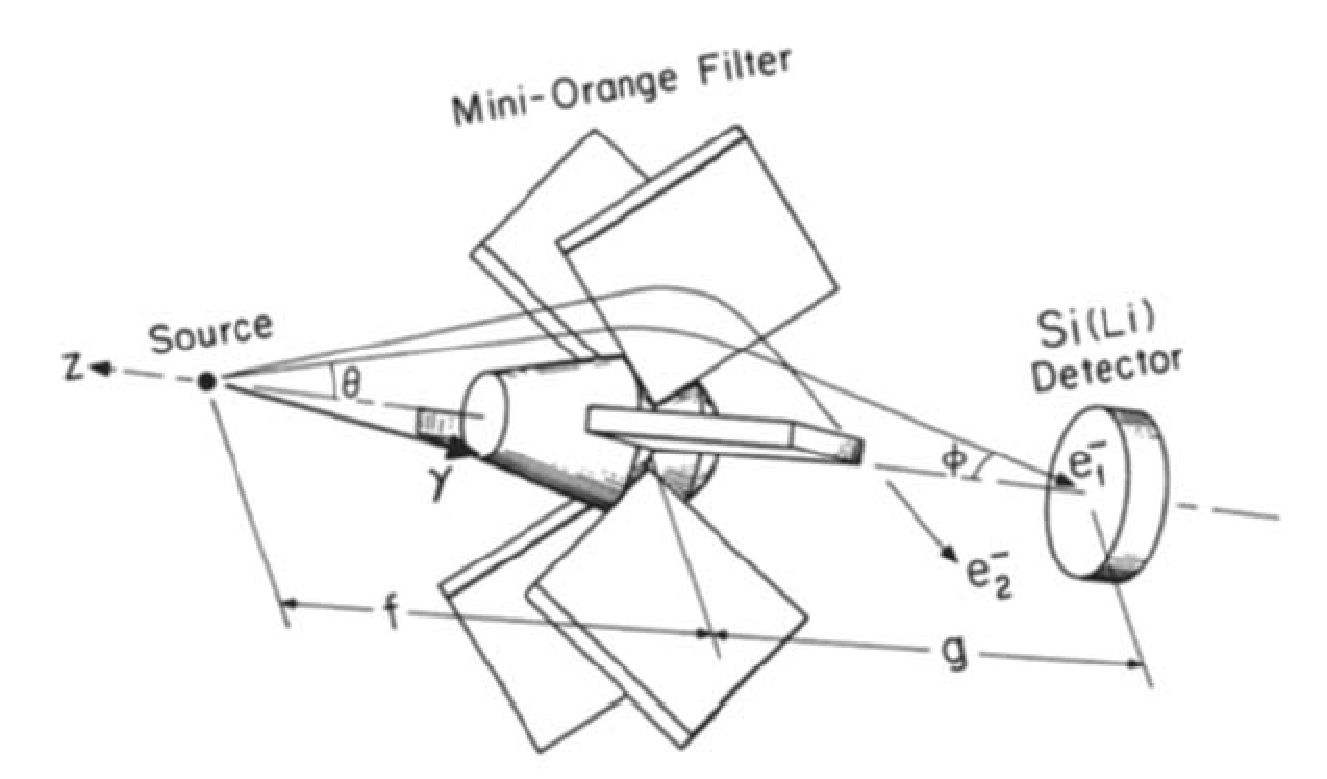
\includegraphics[scale=0.6]{Setup_Figs/mini-orange-metlay-figure.pdf}
    \caption{Graphic of the mini-orange filter. The central blocker keeps $\gamma$-rays from hitting the detector. The magnets bend electrons toward the detectors, and positrons away from the detectors. Being permanent magnets, they are optimized for a range of electron energies, and can cause overbending or underbending of electrons outside of that energy range, making the magnetic filter a factor in the efficiency. Taken from \citep{metlay93:_iceball_comm}}
    \label{fig:mini_orange}
\end{figure}

Compared to conventional spectrometers that sweep over electron energies by changing the magnetic field of the spectrometer, the mini-orange spectrometers are able to cover a wide range of energies at once. A drawback of this is the permanent magnets. The field is optimized for a range of energies, and must be pre-selected before the experiment. Switching magnets mid-experiment is not feasible, due to the downtime needed to warm-up the system, bring it to atmosphere, replace the filter, and then return the system to data taking conditions. Additionally, the efficiency of the system is a convolution of the detector's efficiency and the mini-orange filter in front of it, meaning each configuration must have a separate efficiency measurement. Tables \ref{tab:ICE_Magnet_G} and \ref{tab:ICE_Magnet_C} summarize the magnetic configurations of the mini-orange filters used in the experiments.

\begin{table}[]
    \centering
    \caption{ICEBall magnetic strengths with GEORGINA}
     \label{tab:ICE_Magnet_G}
    \begin{tabular}{c|c|c} \toprule
         Detector & Filter & Strengths \\
         \hline
         1 & M13 & 815,740,830 \\ 
         2 & M15 & 939,911,949\\
         3 & M21 & 850,875,900 \\
         4 & M14 & 972,911,992\\
         5 & M18 & 856,913,963\\
         6 & M22 & 845,900,900\\ \bottomrule
    \end{tabular}
    \\[2]
    \footnotesize
    Magnetic strengths of the mini-orange filters used in the GEORGINA experiments, listed in Gauss. All the magnetic strengths are similar and geared for efficiency peaking at approximately 300-400 keV.
\end{table}

\begin{table}[]
    \centering
    \caption{ICEBall magnetic strengths with Clovershare}
     \label{tab:ICE_Magnet_C}
    \begin{tabular}{c|c|c} \toprule
         Detector & Filter & Strengths \\
         \hline
         1 & M13 & 815,740,830 \\ 
         2 & M20 & 1228,1292,1265\\
         3 & M21 & 850,875,900 \\
         4 & M2 & 1411,1420,1410\\
         5 & M16 & 1286,1340,1285\\
         6 & M22 & 845,900,900\\ \bottomrule
    \end{tabular}
    \\[2]
    \footnotesize
    Magnetic strengths of the mini-orange filters used in the Clovershare experiments, listed in Gauss. The magnetic strengths are mid-energy range and high-energy range for efficiency.
\end{table}

\subsection{Calibration}

ICEBall is calibrated using two sources: $^{133}$Ba and $^{207}$Bi. The specific properties of the two sources are listed in Table \ref{tab:ICE_Cal_Source}. The $^{207}$Bi covers the high-energy regime, with lines around 500 keV and 1000 keV. The $^{133}$Ba covered energies from 200 to 400 keV. Both sources are low activity, preventing incomplete or overlapping charge collection from hindering the resolution of the detectors during calibration runs. 

\begin{table}[]
    \centering
    \caption{ICEBall calibration sources}
        \label{tab:ICE_Cal_Source}
    \begin{tabular}{c|c|c|c|c} \toprule
         Source & Date Measured & Activity & Energy (keV) & Intensity (\%)\\
          \hline 
         $^{133}$Ba & May-4-2012 & 0.331(7) $\mu$Ci & 240.413 & 0.331 \\
         & & & 266.868 & 0.698 \\
         & & & 320.032 & 1.308 \\
         & & & 347.866 & 0.370 \\
         \hline
         $^{207}$Bi & May-4-2012 & 0.306(8) $\mu$Ci & 481.697 & 1.562 \\ 
         & & & 554.4 & 0.469 \\
         & & & 975.657 & 7.243 \\
         & & & 1048.1 & 1.838 \\\bottomrule
    \end{tabular}
    \\[2]
    \footnotesize
    Calibration source information for ICEBall. The energies and the respective intensities are listed for each source. Intensities are taken from \cite{trzaska90:_calibration}. The intensity of the 347 keV line in $^{133}$Ba is both the 384K and 356L intensities combined.
\end{table}

The energy calibration is assumed to be quadratic in nature, although both linear and quadratic calibrations are performed. Figure \ref{fig:iceball_cal} shows both of these fits and their respective residuals for one of the Si(Li) detectors. These values are summarized in the next chapter for each experiment.

\begin{figure}
    \centering
    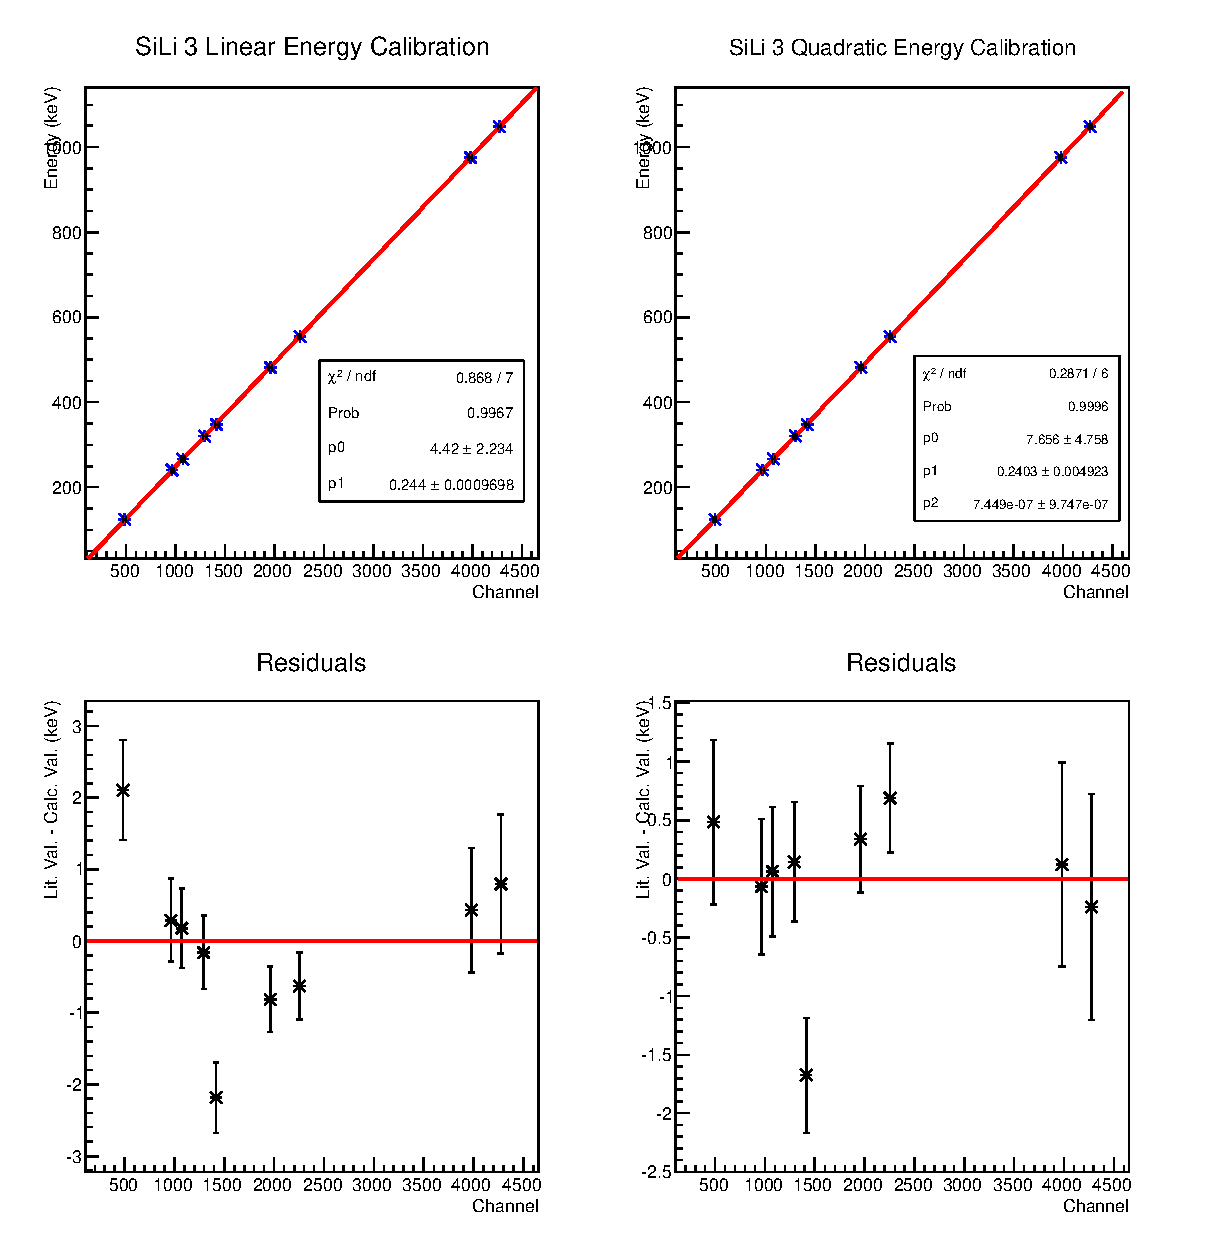
\includegraphics[scale=0.75]{Setup_Figs/sili_3.eps}
    \caption{Linear and quadratic energy calibrations of one Si(Li) detector, using the electron energies listed in Table \ref{tab:ICE_Cal_Source}. The top graphs show the calibrations, while the graphs beneath show the respective residuals. The calibration is in much better agreement in the quadratic fit, as seen in the residuals.}
    \label{fig:iceball_cal}
\end{figure}

The efficiency calibration is fitted to equation

\begin{equation}
    ln(\epsilon) = p_1+p_2ln(E)+p_3E
    \label{eq:SiLi_Eff}
\end{equation}

The efficiency is a convolution of the magnetic configuration and the inherent detector efficiency. Using the efficiency points, the analytic expression for the efficiency was determined empirically in previous work \citep{battaglia15:_iceball_176lu}. These experimental values are summarized in the next chapter for each experiment.

\section{GEORGINA}

GEORGINA is a compact array of high-purity germanium (HPGe) detectors for $\gamma$-ray experiments\citep{isnap18:_georgina}. The detectors are 109\% relative efficiency. These detectors were designed for use with astrophysical capture reactions, meant to cover a large solid angle. There are a total of five detectors.

\subsection{Detectors}

While the GEORGINA detectors were designed for reasonable efficiency up to 12 MeV, they were used in this experiment to look at energies up to 4 MeV. Two detectors of the five were used in this experiment. The detectors were designed with the crystal at a $90^{\circ}$ from the cold-finger, as seen in Figure \ref{fig:georgina}.

\begin{figure}
    \centering
    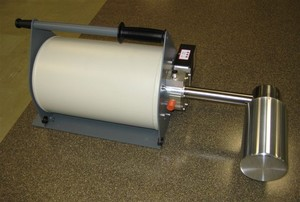
\includegraphics{Setup_Figs/georgina_example.png}
    \caption{An example of one of the GEORGINA detectors. The crystal is at a $90^{\circ}$ from the cold finger, allowing the long side of the crystal to be placed next to the target, to optimize solid angle coverage. In the experiment, the circular face of the crystal was placed toward the target.}
    \label{fig:georgina}
\end{figure}

\begin{table}[]
    \centering
    \caption{GEORGINA Detector Locations}
    \label{tab:GEORGE_Det_Loc}
    \begin{tabular}{c|c|c} \toprule
         Detector & $\theta$ & $\phi$  \\
         \hline
         1 & 0 & 90 \\ 
         2 & 180 & 90\\ \bottomrule
    \end{tabular}
    \\[2pt]
    \footnotesize
    The beam axis is the z-axis. $\theta$ is the angle in the xy-plane, where 0 degrees is beam left. $\phi$ is the azimuthal angle, with respect to the beam axis. All values are in degrees.
\end{table}

One of the two detectors had Bismuth Germanate (BGO) detectors from Argonne National Laboratory around it to cut down on background from incomplete charge collection. BGO detectors have a high efficiency, but poor resolution, and are good to use as a veto system. In the event that a gamma-ray does not deposit its full energy in the HPGe crystal, the BGO detectors surrounding the crystal should pick up the remaining energy. This indicates the event was incomplete in energy and should be excluded from the data. For more on the electronics logic for this, see section \ref{sec:GEORGINA_electronics}.

\subsection{Calibration}

The GEORGINA detectors were calibrated using a $^{152}$Eu source, in addition to the ICEBall sources. The information about the sources is in Table \ref{tab:GEORGINA_Cal_Source}. The $^{152}$Eu source was not designed to sit perfectly on the target ladder, while the two ICEBall sources were. So, even though the Eu source was attached to the target ladder for calibration, using it as a measure of absolute efficiency was not possible. To use the $^{152}$Eu for efficiency, a linear extrapolation of the efficiency of the 344 keV line was done using the 303 keV and 356 keV lines in $^{133}$Ba. All points in the Eu were then scaled based on this. Additionally, several background lines could be used to extend the energy calibration up to 2700 keV. The energy calibration was assumed to be a polynomial, and fits up to the fifth order were done to find the best calibration without overfitting. For examples of these fits and a summary of the determined coefficients, see the next chapter.

\begin{table}[]
    \centering
    \small
    \caption{GEORGINA calibration sources}
    \begin{tabular}{c|c|c|c|c} \toprule
         Source & Date Measured & Activity & Energy (keV) & Intensity (\%)\\
          \hline 
         $^{133}$Ba & May-4-2012 & 0.331(7) $\mu$Ci & 80.997 & 0.3406 \\
         & & & 276.398 & 7.164 \\
         & & & 302.853 & 18.33 \\
         & & & 356.017 & 62.05 \\
         & & & 383.851 & 8.94 \\
         \hline
         $^{207}$Bi & May-4-2012 & 0.306(8) $\mu$Ci & 569.702 & 97.75 \\ 
         & & & 1063.662 & 74.09 \\
         \hline
         $^{152}$Eu & & & 121.7825 & 28.65 \\
         & & & 244.6989 & 7.582 \\
         & & & 344.281 & 26.6 \\
         & & & 411.115 & 2.262 \\
         & & & 443.965 & 3.125 \\
         & & & 778.903 & 13.017 \\
         & & & 867.39 & 4.26 \\
         & & & 964.055 & 14.758 \\
         & & & 1085.842 & 10.062 \\
         & & & 1089.7 & 1.738 \\
         & & & 1112.087 & 13.587 \\
         & & & 1408.022 & 20.945 \\\bottomrule
    \end{tabular}
    \footnotesize
    \item Calibration source information for GEORGINA. The energies and the respective intensities are listed for each source. Intensities are taken from \cite{trzaska90:_calibration}. The  $^{152}$Eu does not have activity and intensity, as it was normalized to the $^{133}$Ba.
    \label{tab:GEORGINA_Cal_Source}
\end{table}

The efficiency calibration is fitted to equation

\begin{equation}
    ln(\epsilon) = a_0-(a_1+a_2\times e^{-a_3\times E})\times E^{-a_4\times E}\times ln(E)
    \label{eq:Ge_Eff}
\end{equation}

This is the same efficiency curve used for the Clovershare detectors, and a characteristic fit can be seen in Figure \ref{fig:clover_eff}. For a summary of the calibration points, please see the next chapter.

\subsection{Electronics and Data Structure}
\label{sec:GEORGINA_electronics}

The data taken with the ICEBall-Georgina pairing of detectors used the electronics set-up from previous experiments\citep{battaglia15:_iceball_176lu}. Signals from the Si(Li), HPGe, and BGO detectors were split into two signals, one for timing and one for energy, as seen in Figure \ref{fig:iceball_electronics}. After going through several NIM (Nuclear Instrumentation Modules) to clean up the signals, these were fed into two VME (Versa Module Europa) bus modules for analog-to-digital conversion. Energy signals were converted using the Mesytec analog-to-digital converter (MADC-32) module. This module has 13 bit resolution. The timing signals were converted using a Caen V778 time-to-digital converter (TDC) module, with 12 bit resolution.

\begin{figure}[hbt!]
    \centering
    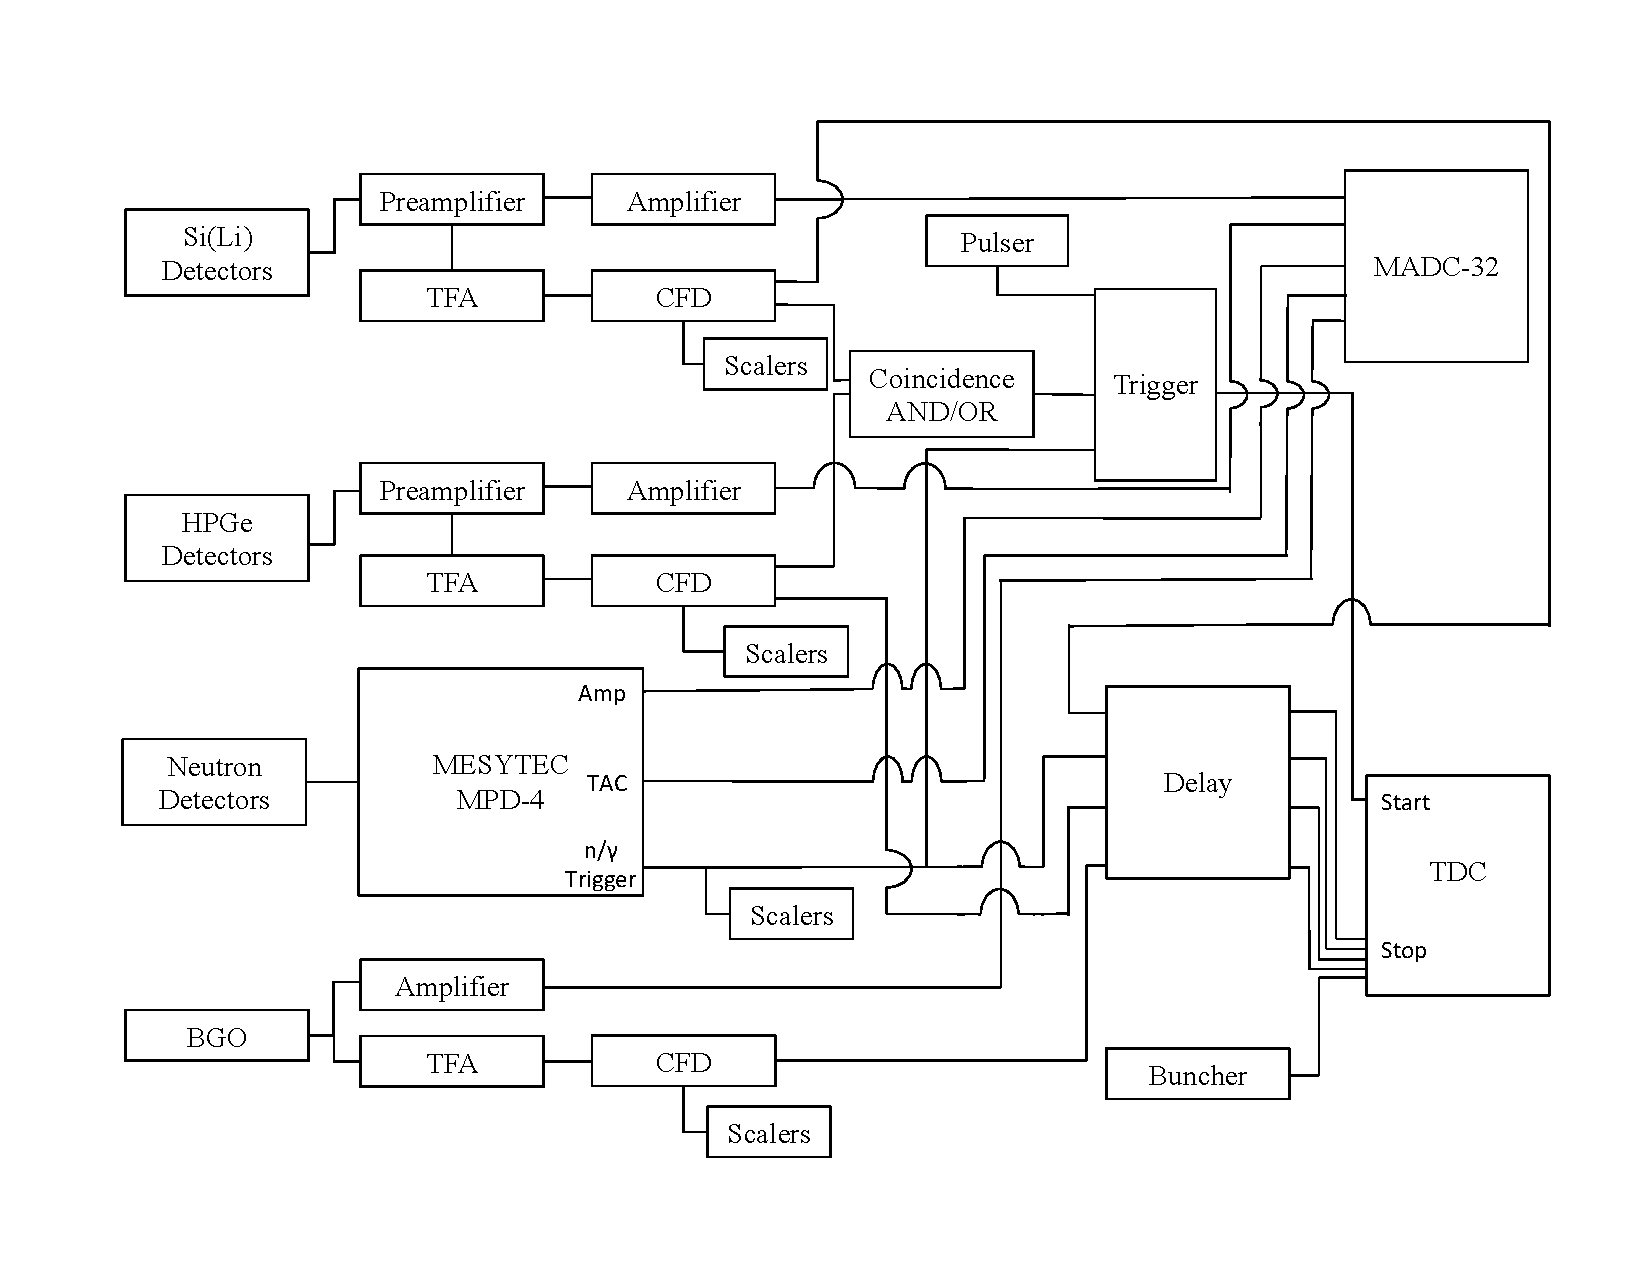
\includegraphics[scale=0.5]{Setup_Figs/electronics-diagram.pdf}
    \caption{A schematic of the electronics for the ICEBall-Georgina set up. See section \ref{sec:GEORGINA_electronics} for a detailed explanation. Taken from \citep{battaglia15:_iceball_176lu}.}
    \label{fig:iceball_electronics}
\end{figure}

The BGO detectors went through an amplifier before being fed directly into the MADC-32. Both the Si(Li)s and the HPGe detectors went into a preamplifier before going into an amplifier, and then the MADC-32. The amplifier allowed for the adjustment of the gain, to optimize the energy regime of interest. The timing signals were sent through a Timing Filter Amplifier (TFA) before going through a constant fraction discriminator (CFD) and being split into start and stop signals, as well as being recorded into the scalers. The stop signal was delayed by \~500ns to prevent self-triggering. Start timing signals were put into a logic coincidence for the trigger. The trigger could be adjusted if the count rate were too high, but the ideal case was the "OR" coincidence, where a Si(Li) or HPGe detector could trigger the start. When this occurred, the signal was sent to a trigger, which sent the TDC a start signal. Stop signals could come from any of the three types of detectors, or the bunched beam being used.

The data was collected from the VME modules using the Michigan State University NSCL data acquisition system (DAQ)\citep{nscl:_daq}. The data file, known as an event or "evt" file, is only compatible with the analysis software SpecTcl\citep{nscl:_daq}. For online analysis, SpecTcl was used. However, for the purposes of gating and fitting, it is inadequate. These evt files were instead converted into "root" files, for use with the CERN Root Data Analysis Framework\citep{brun97:_root}. This open source software is programmable through C++, allowing for a robust set of features. This conversion was done using a program called \texttt{evt2root}\citep{smith14:_evt2root}.

\section{CloverShare}

CloverShare is a group of HPGe clover detectors with BGO shields, that originated at Yale University. They were sent to various laboratories and universities for series of experiments, including the NSL. Two campaigns of experiments were run with CloverShare, each one involving an ICEBall experiment.

\subsection{Detectors}

The CloverShare detectors are large, segmented HPGe detectors, with fitted BGO shields. In the first of the two experiments, 7 detectors were used. In the second, 5 were used, as two experienced pre-amplifier problems during the previous campaign. The detectors used biases between -3000 and -4000 V, and were kept cold using a liquid nitrogen autofill system.

Due to the fixed nature of the ICEBall detectors, the clovers were limited in the angles they could be placed at to optimize efficiency. With the tungsten blockers in front of the Si(Li) detectors to block gamma-rays and x-rays, placing the clovers behind these detectors would drastically reduce efficiency. The system was modeled in AutoDesk Inventor \citep{autodesk:_inventor} to visualize the detector placement, and find an ideal setup to optimize the HPGe detectors. Figure \ref{fig:inventor} shows the resulting model and placements, as well as several unmoveable obstructions, like cable trays, that needed to be worked around.

\begin{figure}[t]
    \centering
    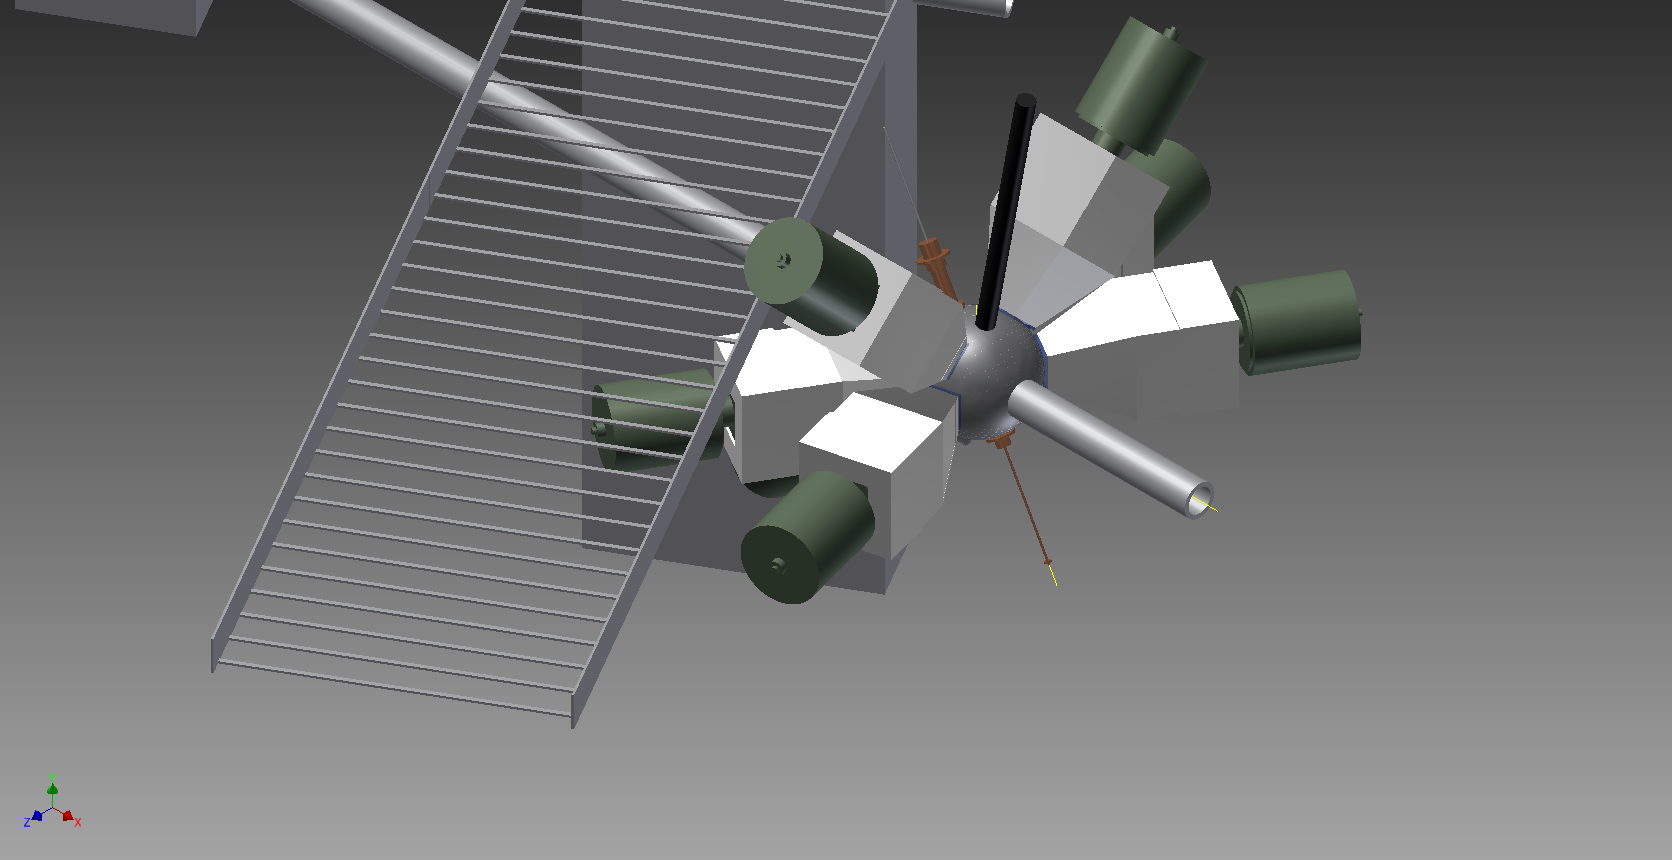
\includegraphics[scale=0.3]{Setup_Figs/FullyAssembled-50cm-newpositions-rightiso.png}
    \caption{ICEBall modeled in Autodesk Inventor \citep{autodesk:_inventor} with the Clovershare detectors placed around it in locations to optimize efficiency. Once ICEBall had been modeled, the detectors were moved around to make sure they were not behind the tungsten blockers. The beamline was also modeled to know where obstructions existed that prevent the Clovershare detectors from being place there.}
    \label{fig:inventor}
\end{figure}

\subsection{Calibration}

The CloverShare detectors were calibrated using the same sources as GEORGINA, as well as at $^{56}$Co source that was created on the FN accelerator days before the experiment. The information about the sources is in Table \ref{tab:GEORGINA_Cal_Source} and \ref{tab:Co_Energy}. 

\begin{table}[t]
    \centering
    \caption{$^{56}$Co Calibration Information}
    \label{tab:Co_Energy}
    \begin{threeparttable}
    \begin{tabular}{c|c}
    \toprule
         Activity & $\gamma$ Energy (keV)  \\ \hline
         6.44 $\mu$Ci\tnote{a} & 846.77 \\
         & 977.372 \\
         & 1037.843 \\
         & 1175.101 \\
         & 1238.288 \\
         & 1360.212 \\
         & 1771.357 \\
         & 2015.215 \\
         & 2034.791 \\
         & 2598.5 \\
         \bottomrule
    \end{tabular}
    \begin{tablenotes}[para]
    Energies used in $^{56}$Co for calibration, as well as activity.
    \newline\item[a] Measured on Mar-16-2016
    \end{tablenotes} 
\end{threeparttable}
\end{table}

The $^{152}$Eu was placed on the individual detectors instead of centered in the trap, as it does not mount well to the target ladder. To use the $^{152}$Eu for efficiency, a linear extrapolation of the efficiency of the 344 keV line was done using the 303 keV and 356 keV lines in $^{133}$Ba. All points in the Eu were then scaled based on this. A characteristic fit of the efficiency of these detectors can be seen in Figure \ref{fig:clover_eff}. A summary of the calibrated efficiency values can be seen in the next chapter.

\begin{figure}[t]
    \centering
    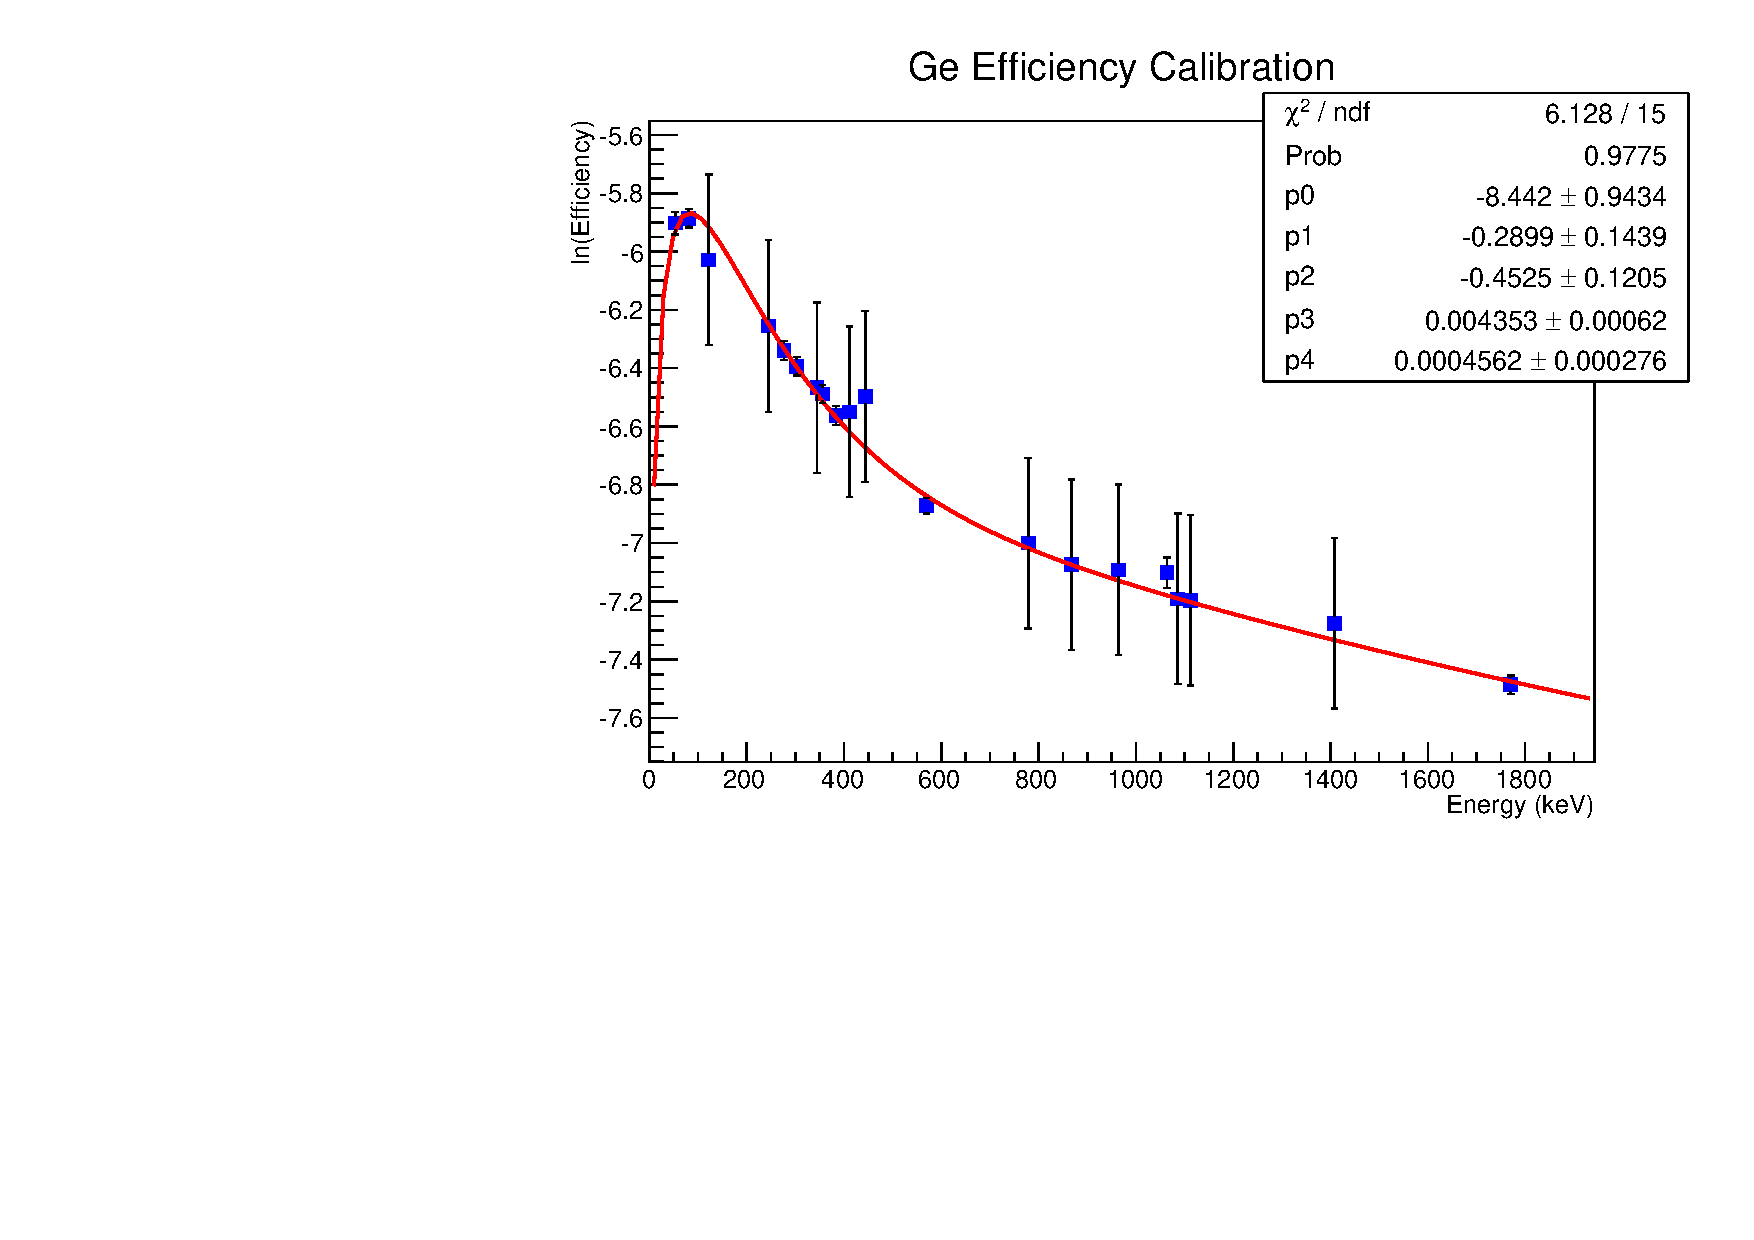
\includegraphics[scale=0.7]{Setup_Figs/Clover1_Eff_05232017.pdf}
    \caption{A characteristic fit of the Clovershare detector efficiencies. The points with large error bars are the $^{152}$Eu points, as the scaling of the points caused a large uncertainty, compared to the $^{207}$Bi and $^{133}$Ba.}
    \label{fig:clover_eff}
\end{figure}

As the clovers are comprised of four separate crystals, the efficiency was taken for the individual leaves, and once the detectors had been calibrated, they were summed together. Figure \ref{fig:Clover_ind_vs_sum} shows the comparison. As is expected, there is a small improvement in the higher energies. The summed crystals were used for analysis, and will be used in spectra from here on forward.

\begin{figure}[hbt!]
    \centering
    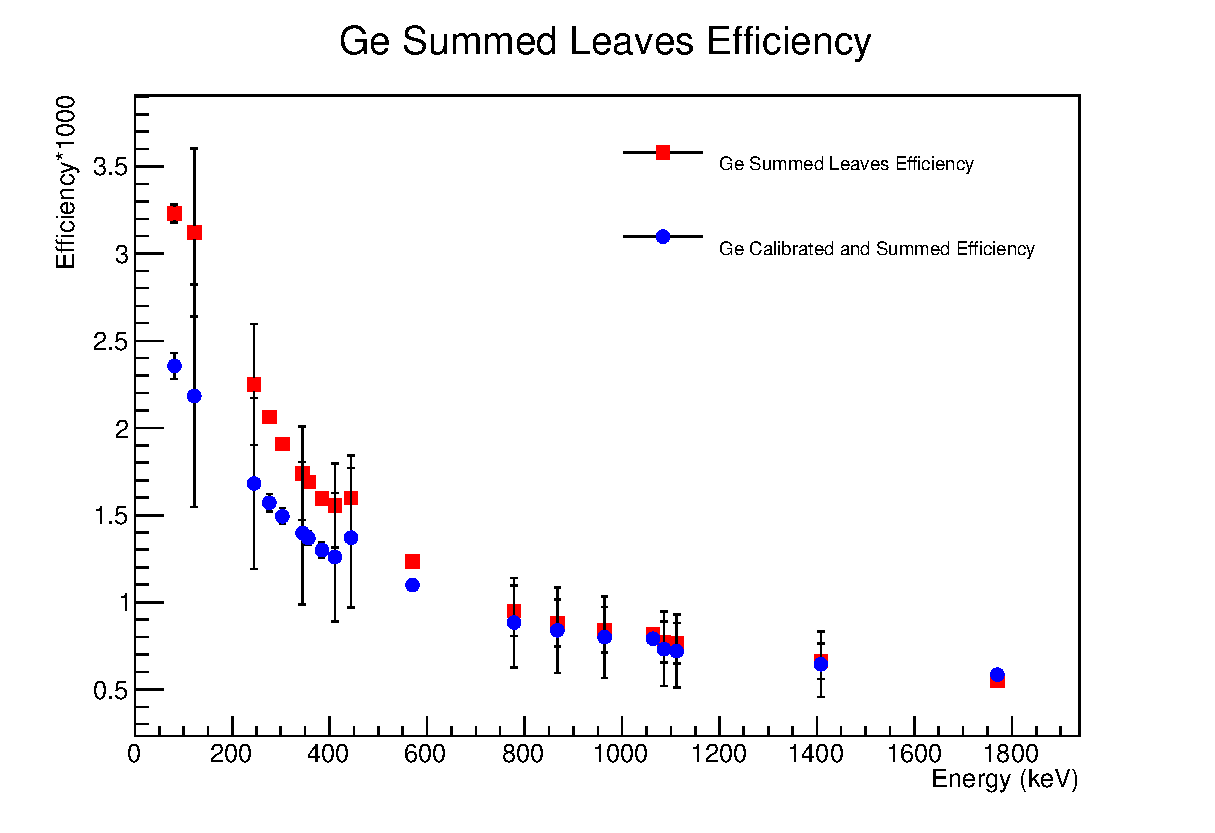
\includegraphics[scale=0.7]{Setup_Figs/Efficiency_ind_vs_sum.eps}
    \caption{Efficiency of a CloverShare detector, with the individual leaves' efficiency summed together, compared to the efficiency of the leaves calibrated and summed together. The different colors/shapes indicate the different sources, as labeled.}
    \label{fig:Clover_ind_vs_sum}
\end{figure}

Each leaf of the clovers was energy calibrated. An unusual trend in the residuals was found in all cases, as seen in Figure \ref{fig:Clover_ene_res}. This trend could not be corrected for by using a higher-order polynomial, as is usually the case for integral non-linearities in multi-channel analyzers \citep{knoll00:rad_det_meas}. Instead, this appears to be a differential non-linearity in the electronics, resulting in discontinuities. As will be discussed in the next section, the electronics used for the experiment are not primarily used with detectors of this sensitivity.

\begin{figure}
    \centering
    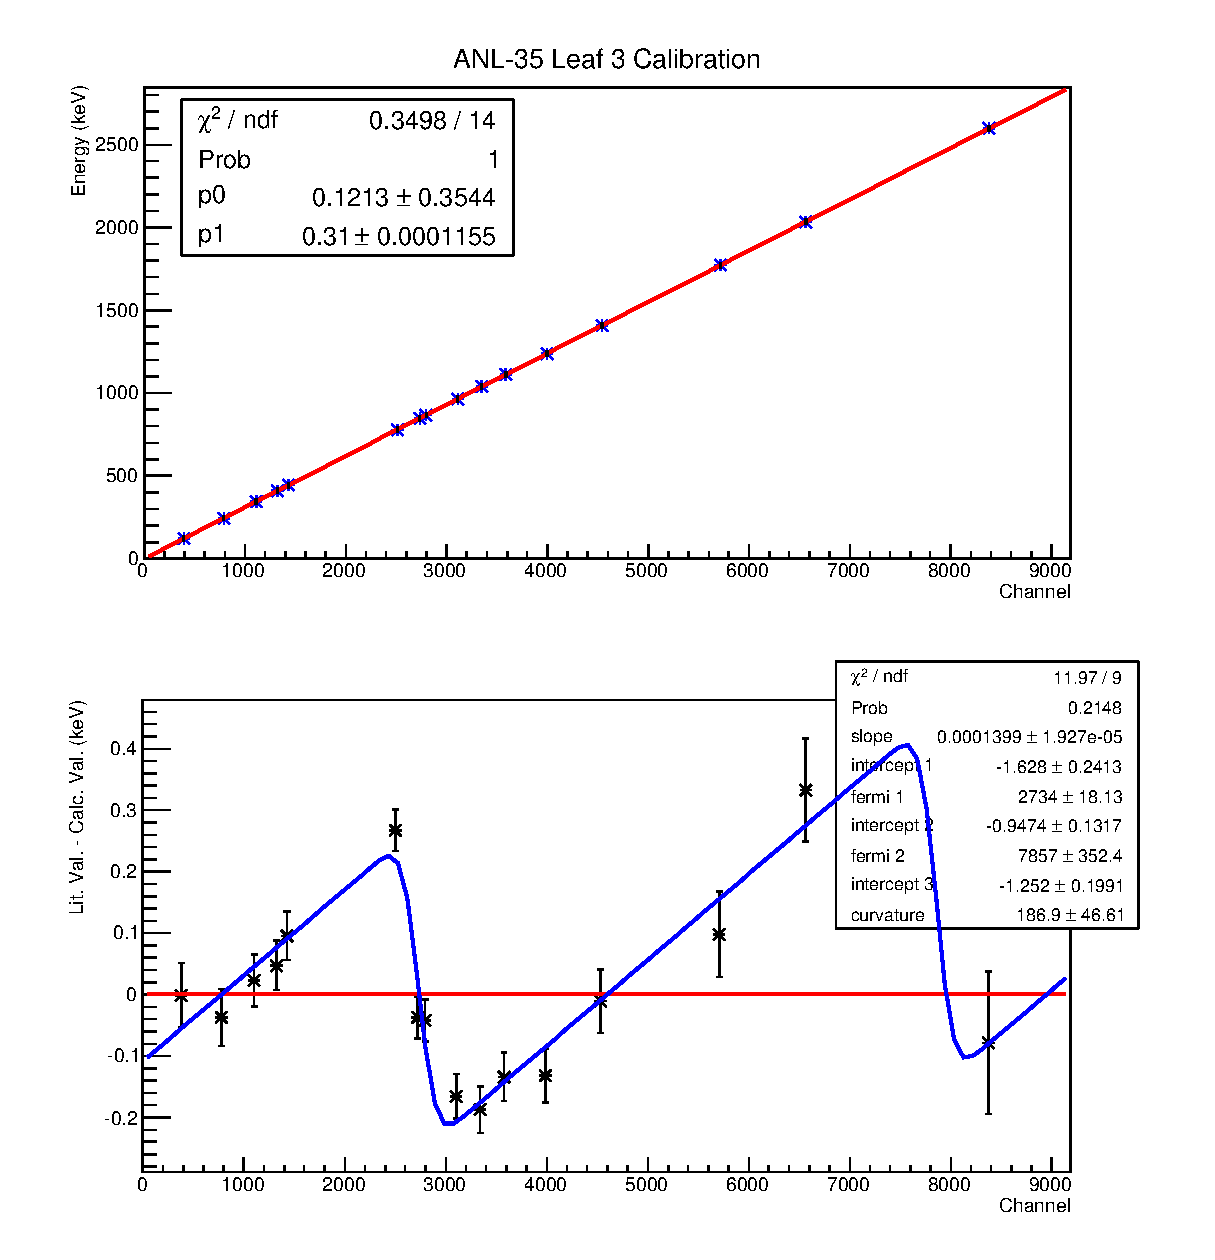
\includegraphics[scale=0.7]{Setup_Figs/Clover_res_cal.eps}
    \caption{A look at the energy calibration of an individual leaf in an HPGe Clover detector. The upper graph is a linear calibration. The lower graph is a look at the residuals. For HPGe detectors, $\pm0.4$ keV is not a good energy calibration. Here, the sawtooth fit that was derived from the differential non-linearity in the electronics is seen fitted to the data.}
    \label{fig:Clover_ene_res}
\end{figure}

\subsection{Electronics}

The electronics used for the Clovershare series of experiments were designed for use with the High Efficiency TOtal absorption spectrometeR (HECTOR), a NaI(Tl) detector array\citep{reingold19:_HECTOR}. The HECTOR data acquisition system is the Michigan Sate University NSCL digital data acquisition system (DDAS). This system uses three XIA Pixie-16 modules \citep{xia:_pixie} which are 16 channel 14-bit 100 MSPS digitizers. Signals from detectors were fed directly from the preamplifiers to the Pixie modules, which did the amplification, shaping, timing, and logic triggers within the module through adjustments on the data acquisition computer. NaI(Tl) detectors have far lower resolution than HPGe detectors, so the differential non-linearities are not noticeable in the HECTOR data.

The Pixie modules were unable to produce enough gain in the amplifier section for the Si(Li) detectors to cover a significant number of channels for resolution, so the detectors' signals were put through fast filter amplifiers \citep{ortec:_fastamp} to boost the signal before being fed into the DDAS. Fast amplifiers were used due to the fast timing and acquisition nature of the Pixie-16 modules and DDAS. 

\section{Beam Production}

Because of the use of HPGe detectors in an $(\alpha,2n)$ reaction, the neutron flux must be minimized in comparison to the cross section of the reaction, as the $(\alpha,n)$ reaction is also open. To do this, a range of energies to test were selected by looking at theoretical cross sections in Talys\citep{koning07:_talys}. These energies were then tested with natural Sm targets, ICEBall, and two liquid scintillators to detect neutrons.

Samarium, as with many even-Z elements in the lanthanide region, has many stable isotopes. A total of five stable isotopes of Samarium exist, with two other isotopes being long-lived. Table \ref{tab:nat_Sm} summarizes the abundances and lifetimes of the various isotopes found in natural Samarium. The two isotopes to be used in enriched targets in the experiments have the highest natural abundances, $^{152,154}$Sm.

\begin{table}[]
    \centering
    \begin{tabular}{c|c|c}
    \toprule
         Isotope & Lifetime (y) & Abundance (\%)  \\
         \hline
         $^{144}$Sm & Stable & 3.08 \\
         $^{147}$Sm & $1.06\times10^{11}$ & 15.00 \\
         $^{148}$Sm & $7\times10^{15}$ & 11.25 \\
         $^{149}$Sm & Stable & 13.82 \\
         $^{150}$Sm & Stable & 7.37 \\
         $^{152}$Sm & Stable & 26.74 \\
         $^{154}$Sm & Stable & 22.74 \\
         \bottomrule
    \end{tabular}
    \caption{Isotope Distribution of Natural Samarium}
    \label{tab:nat_Sm}
\end{table}

\subsection{Talys Calculations}

Talys \citep{koning07:_talys} is software for the simulation of nuclear reactions. Cross sections can be estimated using Talys to guide where an experiment may want to run to optimize production, as is the case presently. 

Both natural and enriched samarium targets were used and modelled within Talys. A range of energies, from 14 MeV to 24 MeV $\alpha$-particles were run. These energies allowed a large number of potential reaction products from elastic, inelastic, transfer, and knockout reactions. Figure \ref{fig:talys} is a visual summary of the strongest modelled reactions in the natural samarium target. It was decided to test the energies between 16-21 MeV.

\begin{figure}[t]
    \centering
    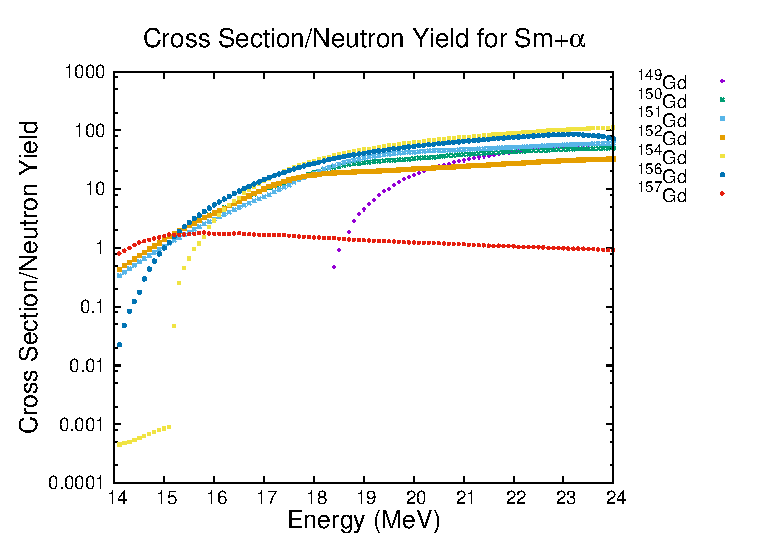
\includegraphics[scale=1]{Setup_Figs/Talys_Ratio.eps}
    \caption{Talys calculation of the highest cross sections divided by the total neutron yield in the natural Samarium target. Only the largest contributors are included, as there are a large number of products possible between the isotopes of Samarium in the target and the reactions channels open for each. All of the largest contributors are Gadolinium isotopes. The ratios for the isotopes of interest appear to plateau around 20-22 MeV.}
    \label{fig:talys}
\end{figure}

\subsection{Test Analysis and Results}

To test these Talys calculations and determine the best running energy, the cross section and neutron flux had to be measured at each energy without the use of the HPGe detectors. ICEBall was used to measure the cross section by examining the K-electrons from ground-state band transitions in the reactions of interest, as the ground-state band is the most significantly populated band in the reaction.

The neutrons were measured using two NE213 liquid organic scintillators. In these detectors, it is possible to do pulse shape discrimination, as the neutrons have longer decay times than the gammas in these detectors due to the nature of the interaction with the scintillating liquid \citep{knoll00:rad_det_meas}. This produces longer trails in the detectors, leading to different decay shapes, see Figure \ref{fig:pulse_discrimination}. 

\begin{figure}
    \centering
    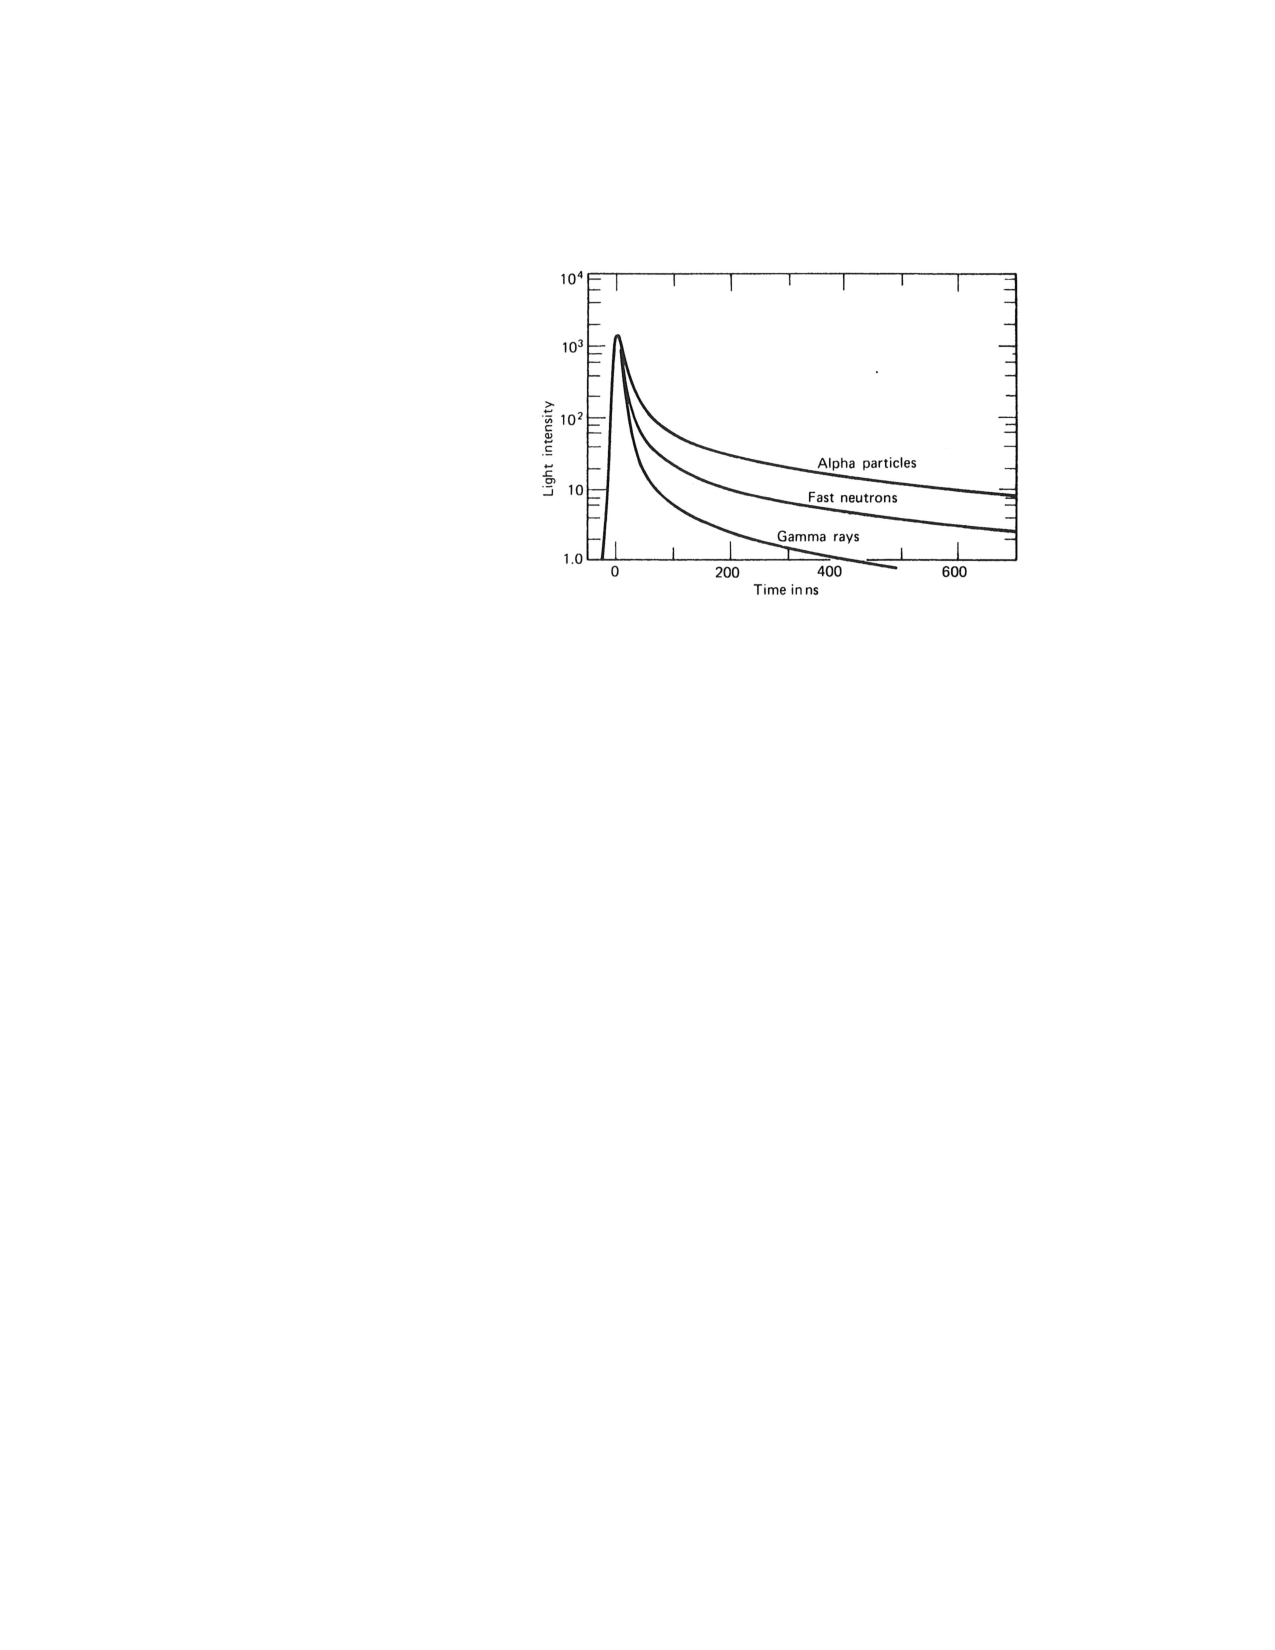
\includegraphics{Setup_Figs/pulse_shape.pdf}
    \caption{A cartoon illustration of pulse shape based on radiation type, in the same detecting material. The different types of radiation interact with the detecting material creating a fast and slow excitation. The ratio of these fast and slow excitations is based on the radiation, and expressed in the length of the decay tail. Picture taken from \citep{knoll00:rad_det_meas}.}
    \label{fig:pulse_discrimination}
\end{figure}

By plotting the pulse height against the decay tail time, neutrons and gammas can be separated. In this setup, this was done by sending the signal to a Mesytec MPD-4 (Multi-channel Pulse Discriminator) \citep{mesytec:_PSD}. This is a module built for pulse discrimination. It splits the signal, amplifies for the pulse height, and sends the other signal to a constant fraction discriminator (CFD), which converts the value to an amplitude using a time to analog converter (TAC). A CFD works by measuring the time it takes for a pulse to decrease to a fraction of its original height. Both of these signals (the pulse amplitude and the TAC amplitude) are recorded in the data. Plotting these values in a two-dimensional plot distinguishes the gammas and neutrons, as in Figure \ref{fig:neutron}. There is a threshold cut off that removed most gammas from the spectrum.

\begin{figure}
    \centering
    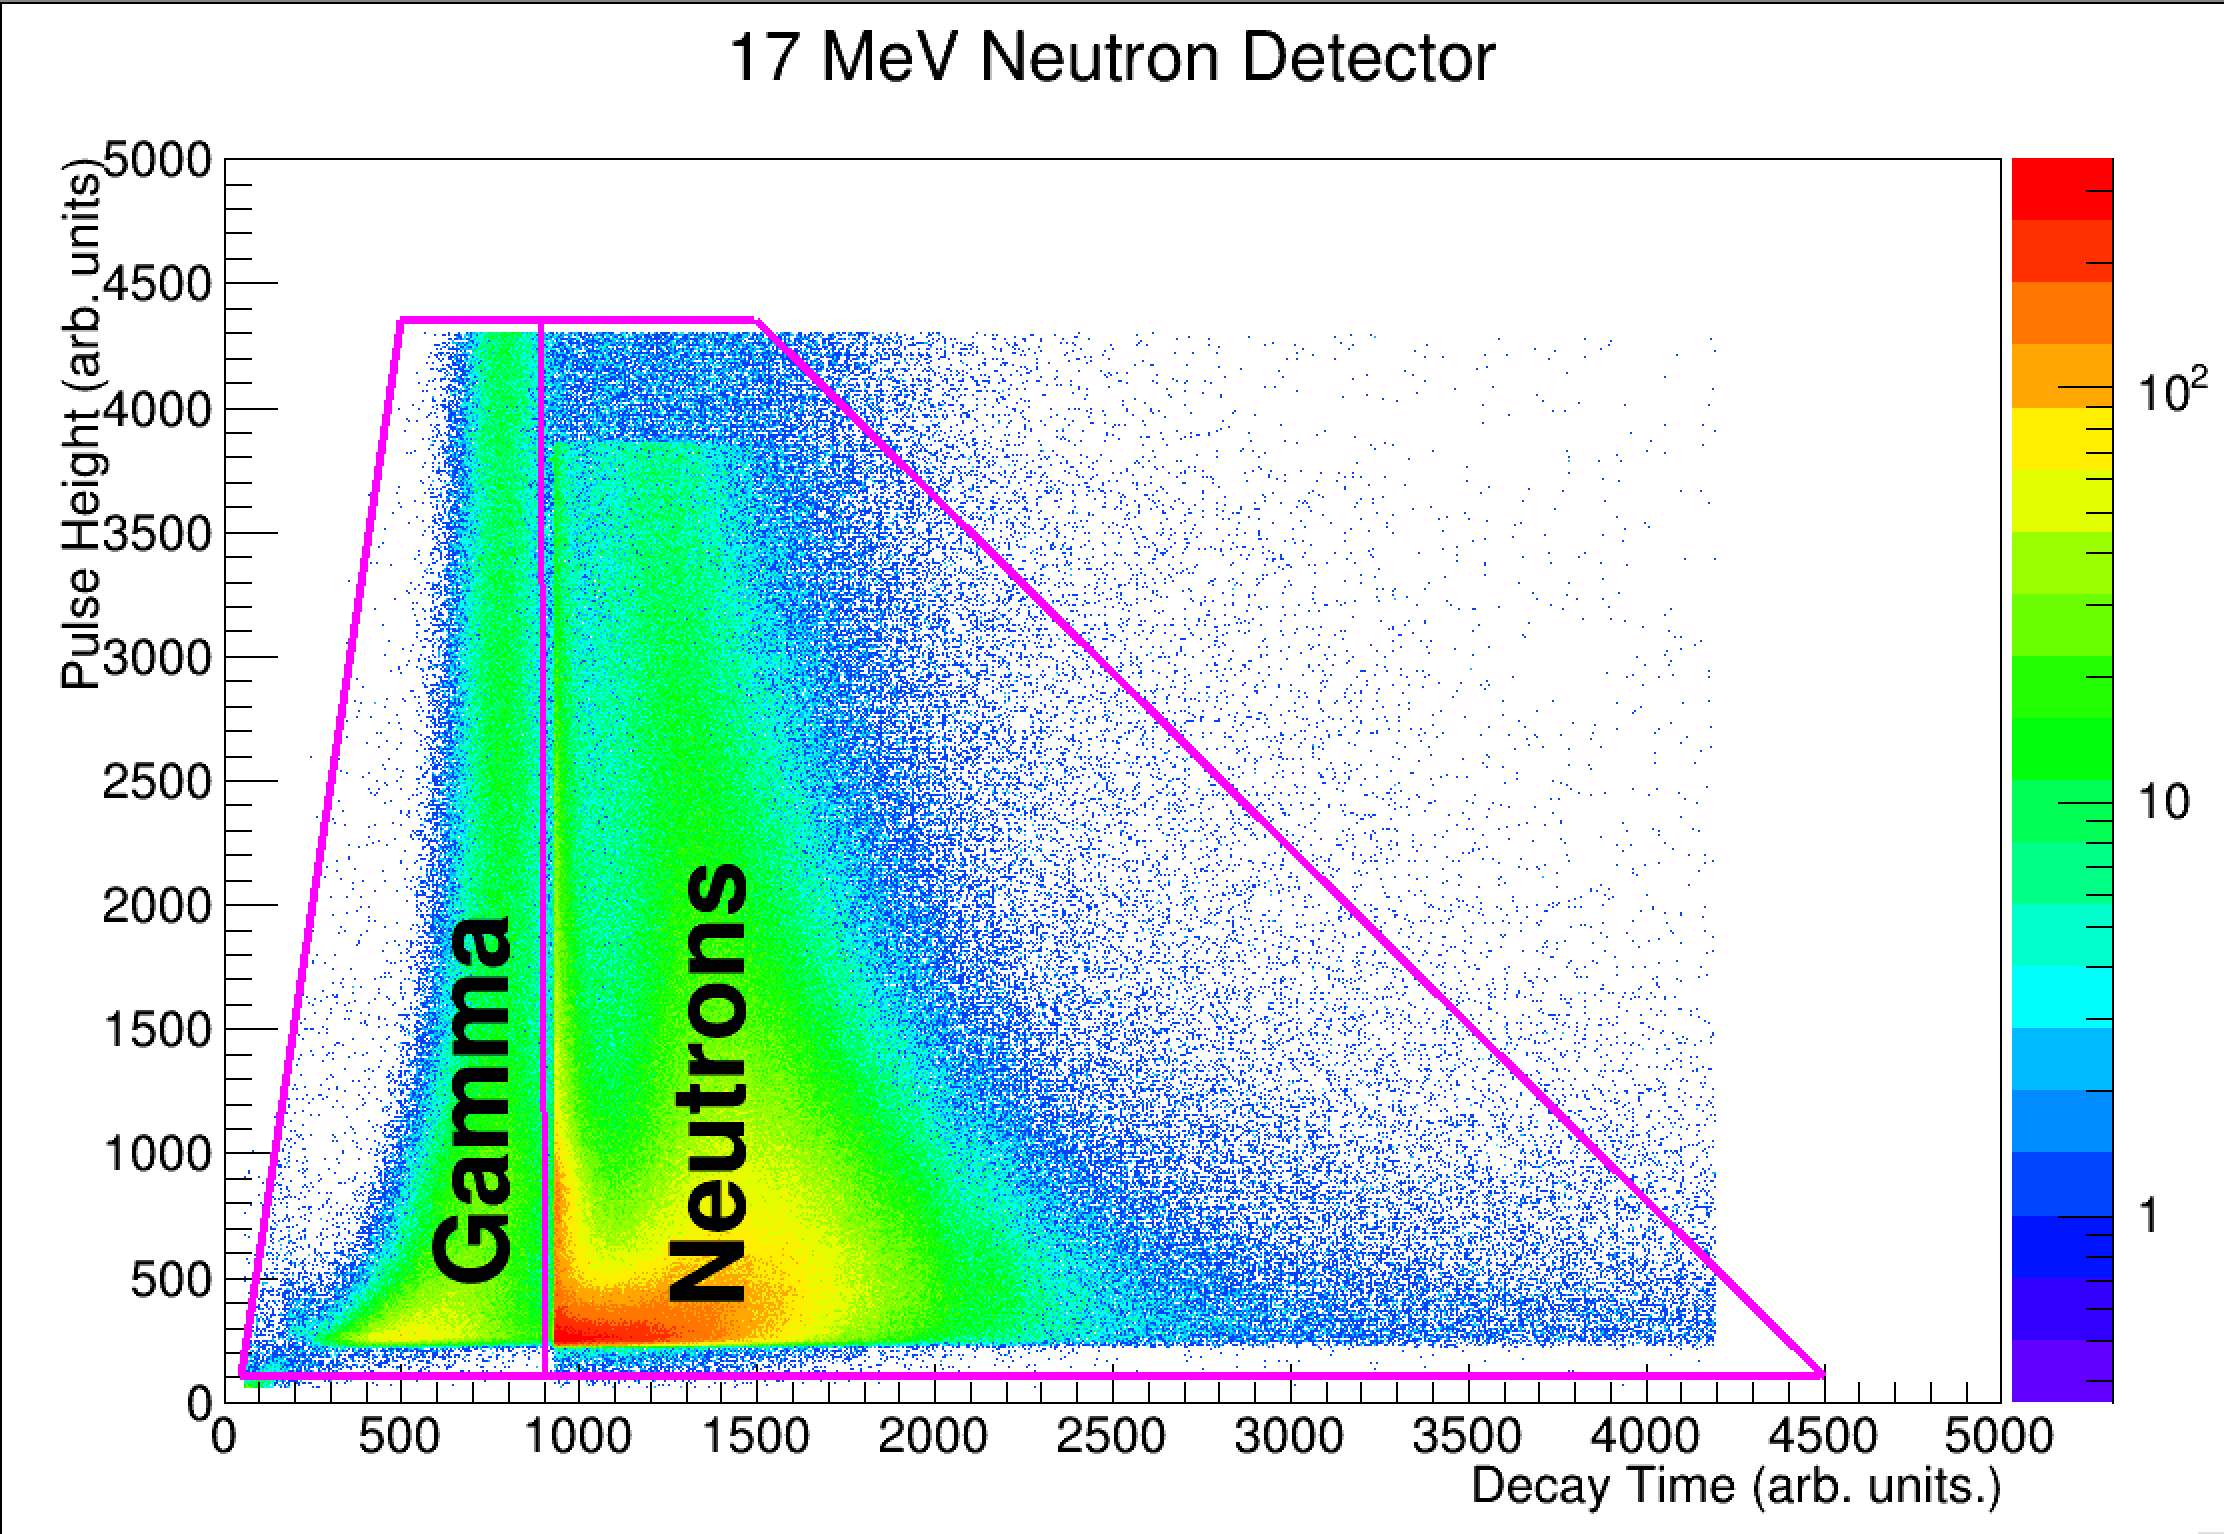
\includegraphics[scale=0.7]{Setup_Figs/17MeVNeutron.eps}
    \caption{Plot of the pulse height vs the decay time in the NE212 detectors. Two clear areas are seen. The leftmost, with the shorter decay time, is the gammas, while the more spread out peak on the right is neutrons.}
    \label{fig:neutron}
\end{figure}

Once the detectors were calibrated, each energy was run, with a total of four different targets across six energies. For each energy, the peaks in the electron spectra were identified with their respective isotopes, working under the assumption that only the lowest-lying states and the ground-state band would be populated significantly enough to see the electrons. These peaks are representative of the reaction cross section for that isotope. The K-electron of the $4^+\rightarrow2^+$ ground state transition for both nuclei of interest was clearly visible and clean at all energies, listed in Table \ref{tab:neutron_electron}. These K-electrons were used for the cross-section calculation.

\begin{table}[]
    \centering
    \caption{$4^+\rightarrow2^+ K-Electrons by Isotope$}
    \begin{tabular}{c|c}
    \toprule
         Isotope & Energy (keV)  \\
         \hline
         $^{154}$Gd & 197 \\
         $^{156}$Gd & 149 
         \bottomrule
    \end{tabular}
    \label{tab:neutron_electron}
\end{table}


To calculate the cross section, the formula

\begin{equation}
    \sigma=\frac{Yield}{\delta x*Q*\epsilon}
    \label{eq:xs}
\end{equation}

was used, where $\delta x$ is the target thickness, $Q$ is the integrated charge, and $\epsilon$ is the efficiency of the Si(Li) detector at the electron energy. The $Yield$ is the area under the curve.

This then had to be compared with the neutron production cross section. A bunched beam was used to get a time-of-flight. Calculating the neutron flux was done using the formula

\begin{equation}
    \sigma_n = \frac{Neutrons}{\delta x*Q}
\end{equation}

where $\delta x$ and $Q$ are the same as used for the cross section. The neutron yield is obtained by pulse shape discrimination, as seen in Figure \ref{fig:neutron}. The left-most line is the gamma-flash that comes from the prompt gammas. The secondary gathering of counts, to the right, is the neutron peak. This area can be integrated over to get the number of neutrons seen during the run.

Table \ref{tab:neutrons} summarizes the results at each energy. Note, that the cross section is not reflective of the full cross section of the isotopes, but of the K-electrons for that transition. This ratio, of the cross-section to the neutron flux, was ultimately used to determine the running energy. The two higher energies, 20 and 21 MeV, have a ratio that agrees within error for both isotopes, indicating a plateau, in agreement with the expectation from Talys. Ultimately, 20 MeV was chosen for two reasons: to minimize any higher energy reaction channels, and because the neutron flux was lower in rate.

\begin{table}[]
    \centering
    \begin{tabular}{c|c|c|c|c|c}
        \toprule
        & \multicolumn{2}{c|}{Cross Section (mb)} & Neutron Flux & \multicolumn{2}{c}{Ratio ($\sigma/\Phi_n$)} \\
        Energy (MeV) & $^{154}$Gd & $^{154}$Gd & (neutrons/s) & $^{154}$Gd & $^{154}$Gd \\
        \hline
        16 & 0.126 (13) & 0.334 (25) & 1.247 (4) & 0.101 (10) & 0.268 (20)\\
        17 & 0.554 (54) & 1.273 (91) & 2.142 (13) & 0.259 (25) & 0.594 (43)\\
        18 & 3.124 (133) & 5.427 (233) & 4.281 (30) & 0.730 (31) & 1.268 (55)\\
        19 & 3.030 (172) & 5.327 (217) & 4.205 (25) & 0.721 (41) & 1.267 (52)\\
        20 & 5.618 (167) & 9.438 (275) & 5.806 (36) & 0.968 (29) & 1.626 (48)\\
        21 & 7.438 (267) & 12.827 (419) & 7.410 (54) & 1.004 (37) & 1.731 (58)\\ 
        \bottomrule
    \end{tabular}
    \caption{Summary of Energy Tests}
    \label{tab:neutrons}
\end{table}

\subsection{Experimental Beam Operation}

The experiments with GEORGINA were done using a bunched beam, creating a set timing signal to help with coincidence. The beam was bunched before the accelerator, with a time separation of 600 ns between bunches. The timing of these bunches is shown in Figure \ref{fig:bunched}. Clear separation in of the bunches is visible.

\begin{figure}
    \centering
    \includegraphics[scale=0.7]{Setup_Figs/Time-of-Flight.eps}
    \caption{This is a plot of the HPGe 1 detector time minus the buncher time. Two distinct peaks can be seen in the spectrum, the main timing peak close to 0, and the much smaller secondary peak, coming from a second bunching signal. The bunching signal only acts as a stop signal for the timing. It can also be used as a veto, as events without a valid buncher time are not real, or are background.}
    \label{fig:bunched}
\end{figure}

% % uncomment the following lines,
% if using chapter-wise bibliography
%
% \bibliographystyle{ndnatbib}
% \bibliography{example}
